%%%%%%%%%%%%%%%%%%%%%%%%%%%%%%%%%%%%%%%%%%%%%%%%%%%%%%%%%%%%%%%%%%%%%%
%%	Name: "Signal analysis template"
%%	File name: signalanalysis_template_main
%%	Version: 1.5
%%
%%	Compiler: XeLaTeX
%%
%%%%%%%%%%%%%%%%%%%%%%%%%%%%%%%%%%%%%%%%%%%%%%%%%%%%%%%%%%%%%%%%%%%%%%

\documentclass[conference,compsoc,onecolumn]{IEEEtran}

% *** LANGUAGE UTILITY PACKAGES ***
\usepackage[utf8]{inputenc} % Required for including letters with accents
\usepackage[spanish]{babel}

% *** USED PACKAGES ***
% *** MISC UTILITY PACKAGES ***
\usepackage{comment}			% Agregar comentarios
\usepackage{lipsum}				% Inserts dummy text
\usepackage{blindtext}
\usepackage{listings}					% Coding
\usepackage{verbatim}				% Verbatim
\usepackage[final]{pdfpages}
\usepackage{booktabs,dcolumn}
\usepackage{pdflscape}
\usepackage{afterpage}
%\setlist[itemize]{noitemsep, nolistsep}
\usepackage[bookmarks=false]{hyperref}
\usepackage{tcolorbox}									% Coloured boxes, for LATEX examples and theorems, etc
\usepackage{color}
\usepackage{xcolor} % Required for specifying colors by name									% Color packages foreground and back­ground color man­age­men
% *** CITATION PACKAGES ***
\usepackage{cite}
% *** GRAPHICS RELATED PACKAGES ***
\usepackage{graphicx}
\usepackage{caption}
\usepackage{pgfplots}
\usepackage{tikz}
\usetikzlibrary{shapes,arrows}
\usetikzlibrary{decorations.pathmorphing} % noisy shapes
\usetikzlibrary{fit}					% fitting shapes to coordinates
\usetikzlibrary{backgrounds}	% drawing the background after the foreground
\pgfplotsset{compat=1.13}
% *** MATH PACKAGES ***
\usepackage{amsmath}
\usepackage{mathtools}
\usepackage{amssymb}
\usepackage{amsfonts}
\usepackage{expl3}
\usepackage{bm}

% *** SPECIALIZED LIST PACKAGES ***
\usepackage{algorithmic}
\usepackage{listings}					% Coding
\usepackage[framed,numbered,autolinebreaks,useliterate]{mcode}
% *** ALIGNMENT PACKAGES ***
\usepackage{array}
% *** SUBFIGURE PACKAGES ***
%\ifCLASSOPTIONcompsoc
%\usepackage[caption=false,font=normalsize,labelfont=sf,textfont=sf]{subfig}
%\else
%\usepackage[caption=false,font=footnotesize]{subfig}
%\fi
% *** FLOAT PACKAGES ***
\usepackage{fixltx2e}
\usepackage{stfloats}
%\fnbelowfloat
%\usepackage{dblfloatfix}
% *** PDF, URL AND HYPERLINK PACKAGES ***
\usepackage{url}
\usepackage{everypage}


\usepackage{multirow} % In order to be able to insert rows spanning multiple lines
\usepackage{verbatim}
\usepackage[all]{xy}
\usepackage{listings}
\usepackage{subfigure}
\usepackage{multibib}
\usepackage{setspace} 
\usepackage{algorithm}			    	  % To insert nice algorithms

% *** CARPETA DONDE SE GUARDARAN LAS IMAGENES ***
\graphicspath{{figures/}}

% *** NUEVOS COMANDOS Y CONFIGURACIONES VARIAS ***
\interdisplaylinepenalty=2500
\newcommand{\Lpagenumber}{\ifdim\textwidth=\linewidth\else\bgroup
	\dimendef\margin=0
	\ifodd\value{page}\margin=\oddsidemargin
	\else\margin=\evensidemargin
	\fi
	\raisebox{\dimexpr -\topmargin-\headheight-\headsep-0.5\linewidth}[0pt][0pt]{%
		\rlap{\hspace{\dimexpr \margin+\textheight+\footskip}%
			\llap{\rotatebox{90}{\thepage}}}}%
	\egroup\fi}

\AddEverypageHook{\Lpagenumber}%

\newcommand{\newtxt}[1]{\textcolor{black}{#1}}
\renewcommand\IEEEkeywordsname{Palabras cláve:}
\newcommand{\mx}[1]{\mathbf{\bm{#1}}} % Matrix command
\newcommand{\vc}[1]{\mathbf{\bm{#1}}} % Vector command

%% Separación de palabras
\hyphenation{op-tical net-works semi-conduc-tor HHMMSS}


\begin{document}

% *** TITLES AND NAMES ***
% title of the document
\title{Plataforma de seguimiento de datos COVID-19 para Colombia}
% author names and affiliations

\makeatletter
\newcommand{\linebreakand}{%
  \end{@IEEEauthorhalign}
  \hfill\mbox{}\par
  \mbox{}\hfill\begin{@IEEEauthorhalign}
}
\makeatother

\author{
    \IEEEauthorblockN{Janis~Andrea~Salazar~Sánchez}
    \IEEEauthorblockA{Escuela de Ciencias Exactas e Ingeniería\\
	    Universidad Sergio Arboleda - Bogotá, Colombia\\
	    janis.salazar01@correo.usa.edu.co}
    \and
    \IEEEauthorblockN{Valeria~Carvajal~Romero}
    \IEEEauthorblockA{Escuela de Ciencias Exactas e Ingeniería\\
	    Universidad Sergio Arboleda - Bogotá, Colombia\\
	    valeria.carvajal01@correo.usa.edu.co}
    \linebreakand
    \IEEEauthorblockN{Michael~Steven~Pinilla~Mateus}
    \IEEEauthorblockA{Escuela de Ciencias Exactas e Ingeniería\\
	    Universidad Sergio Arboleda - Bogotá, Colombia\\
	    michael.pinilla01@correo.usa.edu.co}
    
}

% *** MAKE TITLE ***
\maketitle
\IEEEoverridecommandlockouts
\IEEEpeerreviewmaketitle

\begin{abstract}
Como entrega de la primera parte del proyecto de aula del curso Análisis de señales se desarrolla una plataforma que extrae los datos actualizados del COVID-19 presentados en
Colombia, tomando estos datos de la pagina web de datos del gobierno 'Datos Abiertos del Coronavirus COVID-19 por ciudad en Colombia', y los guarda en una base de datos. Los datos posteriormente se representan
de forma selectiva mediante gráfica circular, gráficos de dos dimensiones y diagramas de barras. En este desarrollo se utiliza el lenguaje de programación python y el sistema de gestión de bases de datos SQLite.

\end{abstract}


\begin{IEEEkeywords}
COVID-19, Colombia, plataforma, seguimiento, pandemia
\end{IEEEkeywords}

\section{Antecedentes}
Dar cara a la pandemia ha sido un desafío para el sector de la salud y la epidemiología, para el personal que trabaja en primera línea y los que derivan en todo el mundo. La poca certidumbre, la atención dedicada a cada paciente y la precoz infraestructura y herramientas, los intentos de conseguir resultados e intervenciones optimos, la ansiedad, miedo y preocupacación colectiva, el desconocimiento sobre las consecuencias futuras en el organismo, además a la probabilidad que existe de muerte incrementa el pánico al contagio, que al dia de hoy, 30 de septiembre del año 2020, se registra en Colombia el SARS-CoV-2  como la segunda causa de muerte. 
\medskip
Se tiene evidencia que el pulmón es uno de los órganos con mayor riesgo de sufrir complicaciones cronicas, donde hay perturbaciones en el proceso respiratorio, afectando la capacidad de realizar ejercicio, las necesidades de oxígeno y la calidad de vida. El "volver a la normalidad" que varios anhelan es una esperanza con muy bajas probabilidades de que ocurra. 
\label{sec:results}

\section{Bibliotecas utilizadas}
A continuación se describe brevemente las bibliotecas utilizadas en el desarrollo de la plataforma:

 \begin{table}[H]
    \centering
    \begin{tabular}[c]{| m{15em} | m{35em} |} 
     \hline
     \textbf{Biblioteca} & \textbf{Utilidad}\\
     \hline
      \textit{pandas} & Manipulación y análisis de datos para el lenguaje de programación Python. En particular, ofrece estructuras de datos y operaciones para manipular tablas y series temporales.\\ 
     \hline
      \textit{sqlite3} & Biblioteca con funciones que permiten gestionar una base de datos liviana que proporciona un sistema de administración para bases de datos relacionales y sin mucha configuración.\\
     \hline
      \textit{matplotlib.pyplot} & Es una colección de funciones de estilo comando que hacen que matplotlib funcione como MATLAB. Cada función pyplot realiza algún cambio en una figura: Por ejemplo, crea una figura, crea un area de trazado en una figura, traza algunas líneas en un area de trazado, decora el trazado con etiquetas, etc.  \\ 
     \hline
      \textit{os} & Proporciona funciones para interactuar con el sistema operativo. OS, viene bajo los módulos de utilidad estándar de Python. Este módulo proporciona una forma portátil de utilizar la funcionalidad dependiente del sistema operativo. \\
     \hline
    \end{tabular}
    \caption{Bibliotecas utilizadas de python en el desarrollo.}
    \label{table:ta}
    \end{table}

\label{sec:results}

\section{Resultados}
Como se puede observar en la siguiente gráfica se estima porcentualmente en que estado se encuentran las personas contagiadas por COVID-19 en Colombia, donde una gran parte de estas han logrado recuperarse con un porcentaje del 89.3\% del total de casos. A pesar de que los recuperados son una cifra significativa, esto no representa que sean inmunes o que no puedan volver a contagiarse, además de que aún no se tiene información de si puedan llegar a presentar secuelas u dolencias crónicas. El 5.6\% se encuentran en aislamiento obligatorio en sus casas mientras su organismo logra eliminar el virus. El 1.9\% están siendo atendidos por el personal de salud en centros hospitalarios donde un 0.2\% se encuentran gravemente, siendo atendidos en la unidad de cuidados intensivos (UCI). Aunque el porcentaje de fallecidos se pueda considerar bajo, del 3.1\%, hay que ser conscientes de que se habla de vidas, un total de 25,998 personas que han dejado de estar con nosotros.\\

\begin{figure}[H]
\centering
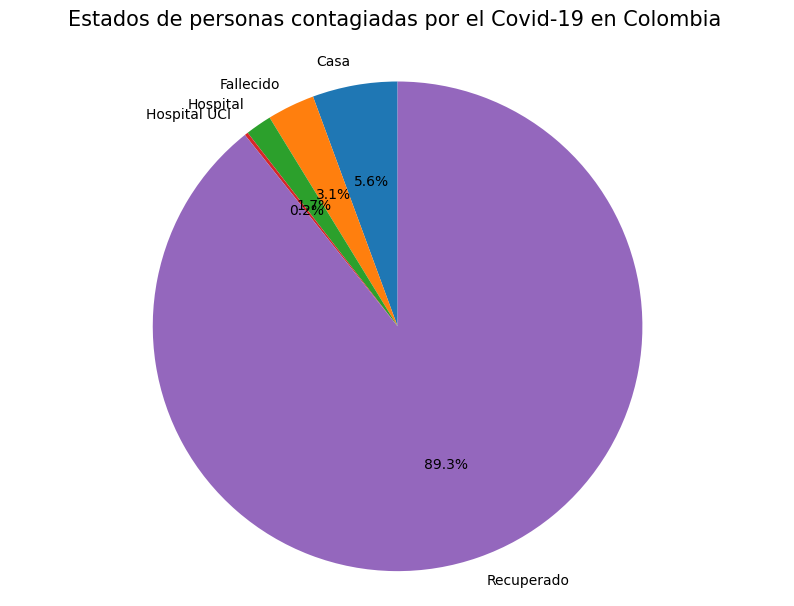
\includegraphics[width=10cm]{./images/GraficaCircular_Estados.png}
\caption{Gráfica circular del estado de las personas con COVID-19 en Colombia}
\label{fig:mesh1}
\end{figure}
En la siguiente figura se puede evidenciar de manera clara la diferencia presentada entre la población de hombres y mujeres que se encuentran infectados actualmente de COVID-19 en Colombia, los valores se observan de manera porcentual y como resultado podemos concluir que la población masculina presenta mayores casos activos en un pequeño porcentaje de diferencia.\\
\begin{figure}[H]
\centering
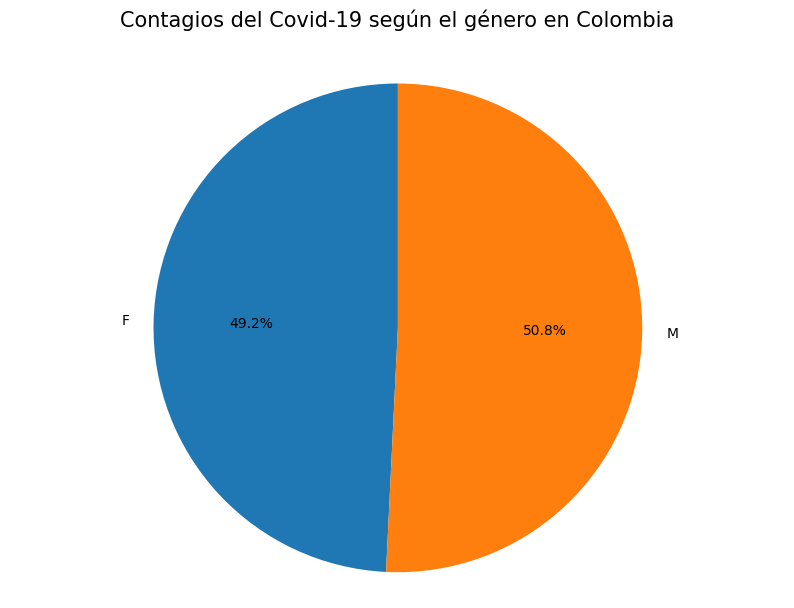
\includegraphics[width=9cm]{./images/GraficaCircular_Genero.png}
\caption{Gráfica circular de personas contagiadas con COVID-19 en Colombia según el sexo}
\label{fig:mesh1}
\end{figure}

Ahora, se representa a través de una gráfica de barras la cantidad de personas fallecidas clasificadas por su edad. Los contagiados que tuvieron una edad entre los 60 a 90 años de edad al momento de fallecimiento representan la mayoría, dando a entender que en este sector de la población existe una mayor tasa de letalidad en comparación con grupos de menor edad, representando una población más vulnerable. Aunque la mayor tasa de letalidad está en una edad avanzada, no quita la probabilidad de que niños, adolescentes, adultos jovenes y adultos estén en riesgo de morir por el virus del COVID-19.  \\
\begin{figure}[H]
\centering
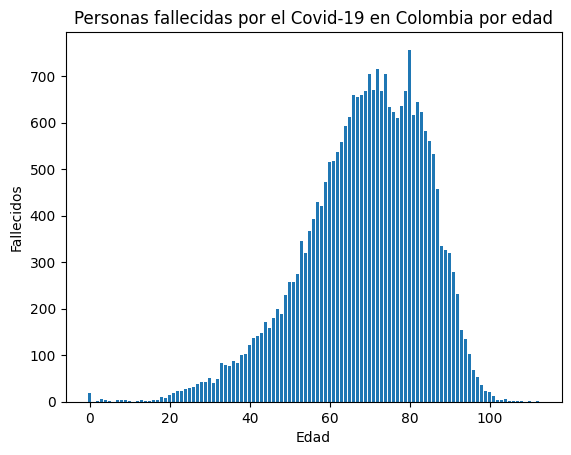
\includegraphics[width=10.5cm]{./images/GraficoBarras_Edad_Fallecidos.png}
\caption{Gráfica de barras de fallecimientos por COVID-19 en Colombia según la edad}
\label{fig:mesh1}
\end{figure}

A continuación, se tiene la gráfica de barras donde se realiza una comparación entre dos etnias, la indígena y la negra, obteniendo que mayormente hay contagiados en la etnia negra, casi a representar el doble de la indígena. Sin tener información relevante del porqué la etnia indígena conserva una cantidad minoritaria de contagiados, se puede aventurar a suponer que es debido a que su población es menor, ya que en Colombia ciertos grupos ilícitos y personal gubernamental toman como blanco de tiro a esta etnia.
\begin{figure}[H]
\centering
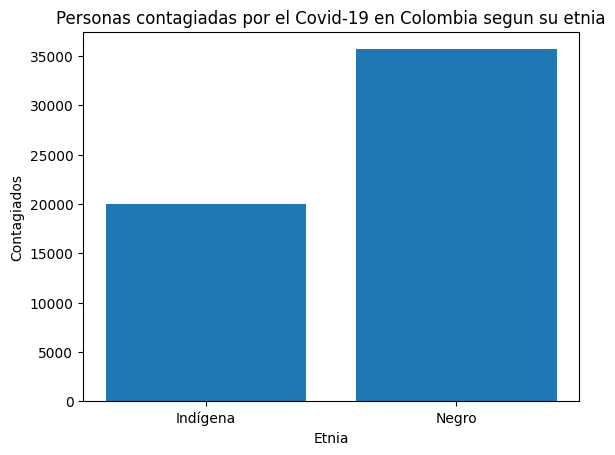
\includegraphics[width=10.5cm]{./images/GraficoBarras_Etnia_Contagios.png}
\caption{Gráfica de barras de contagiados por COVID-19 en Colombia según la etnia}
\label{fig:mesh1}
\end{figure}

En cuanto a los contagios por edad, se realiza una gráfica de dos dimensiones para visualizar la información, obteniendo que existe un mayor contagio en personas que rondan las edades entre los 30 a 50 años. Aunque este sector de la población representa la mayor tasa de contagio, no se llevan el título de mayor tasa de letalidad.

\begin{figure}[H]
\centering
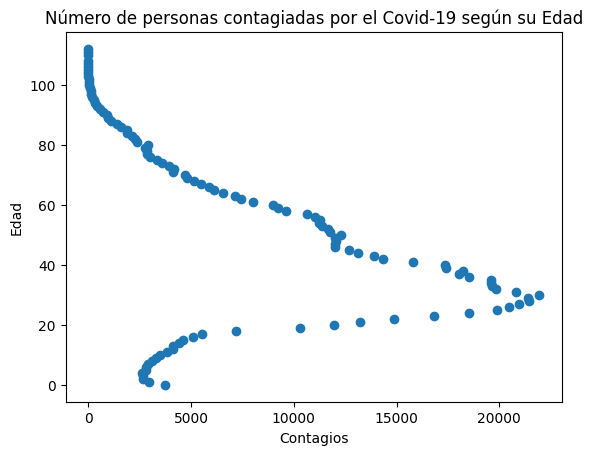
\includegraphics[width=10cm]{./images/Grafico2d_Edad.png}
\caption{Gráfica 2D de contagiados por COVID-19 en Colombia según la edad}
\label{fig:mesh1}
\end{figure}

Para finalizar, se hace un análisis más localizado en el departamento de Vichada, obteniendo que en sus principales 4 ciudades (Santa Rosalía, Puerto Carreño, La Primavera y Cumaribo) existe un muy bajo número de contagiados reportados, excepto en su capital, Puerto Carreño, que si resalta entre sus vecinas con un número de aproximadamente 400 contagios.  

\begin{figure}[H]
\centering
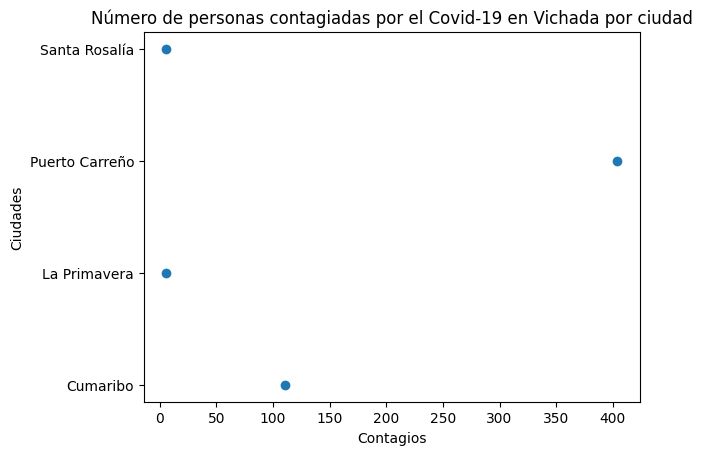
\includegraphics[width=10cm]{./images/Grafico2d_Vichada.png}
\caption{Gráfica 2D de contagiados por COVID-19 en Colombia localizados en las ciudades del departamento de Vichada}
\label{fig:mesh1}
\end{figure}

\label{sec:results}




\section{Conclusiones}
A continuación se resume las conclusiones basadas en los resultados obtenidos: 
\label{sec:conclusions}
\begin{itemize}
    
    \item La población masculina presenta mayores casos activos en un pequeño porcentaje de diferencia respecto a las mujeres.
    \item Los contagiados que tienen una edad entre los 60 a 90 años de edad tienen la mayor tasa de letalidad en comparación con grupos de menor edad. 
    \item Una gran parte de personas han logrado recuperarse del COVID-19 con un porcentaje del 89.3\% del total de casos. El 5.6\% se encuentran en aislamiento obligatorio. El 1.9\% están siendo atendidos por el personal de salud en centros hospitalarios donde un 0.2\% se encuentran en UCI y el porcentaje de fallecidos es del 3.1\%.
    \item Entre las etnias indígena y negra, existe mayor número de contagios en la etnia negra, casi representando el doble de la indígena.
    \item Las personas que rondan las edades entre los 30 a 50 años representa la mayor tasa de contagio.
    \item En el departamento de Vichada existe un muy bajo número de contagiados reportados, excepto en su capital, Puerto Carreño.
    
\end{itemize}

\section{Repositorio GIT}
En el siguiente link se encuentra el repositorio GIT que se utilizó para el desarrollo de la plataforma:
\begin{itemize}
\item https://github.com/Vaal-01/COVID-Colombia
\end{itemize}

\nocite{*}
\bibliographystyle{IEEEtran}
\label{sec:biblio}
% Descomente y modiffique el archivo biblio.bib para agregar bibliografía
\bibliography{bib/biblio} 





%\pagestyle{empty}
\end{document}

